\chapter{Lineare Bauteile}

\section{Kondensator}

\subsection{Kapazität}

\subsection{Ladung}

\section{Spule}

\subsection{Induktionsvorgänge}

\subsection{Kopplungsgrad}

\subsection{Induktivitäten}

\section{RLC Netzwerke}

\subsection{$\tau$-Messung}

\section{Resonanzkreise}

\subsection{Güte}

\subsection{Bandbreite}

\section{Übertragungsfunktion}
Die Übertragungsfunktion beschreibt das Ausgangs- im Vergleich zum
Eingangssignal und ist definiert als
\begin{align}
    \underline{H}(j\omega)=\frac{\underline{U}_2}{\underline{U}_1}
\end{align}
wobei $\underline{U}_1$ der Eingang und $\underline{U}_2$ der Ausgang ist.

\subsection{Bodediagramm}
Das Bodediagramm zeigt das Verhalten eines Systems im logarithmischen
Frequenzbereich. Es besteht aus Amplitudengang (in dB) und Phasengang (in °)
und veranschaulicht die Übertragungsfunktion $H(j\omega)$.\\\\ Der
\textbf{Amplitudengang} zeigt, wie stark ein System das Ausgangssignal im
Vergleich zum Eingangssignal bei verschiedenen Frequenzen verstärkt oder
abschwächt. \\ Der \textbf{Phasengang} zeigt die Verzögerung oder Voreilung des
Ausgangssignals im Vergleich zum Eingangssignal bei verschiedenen Frequenzen.
\\\\ \textbf{Amplitudengang:}
\begin{center}
    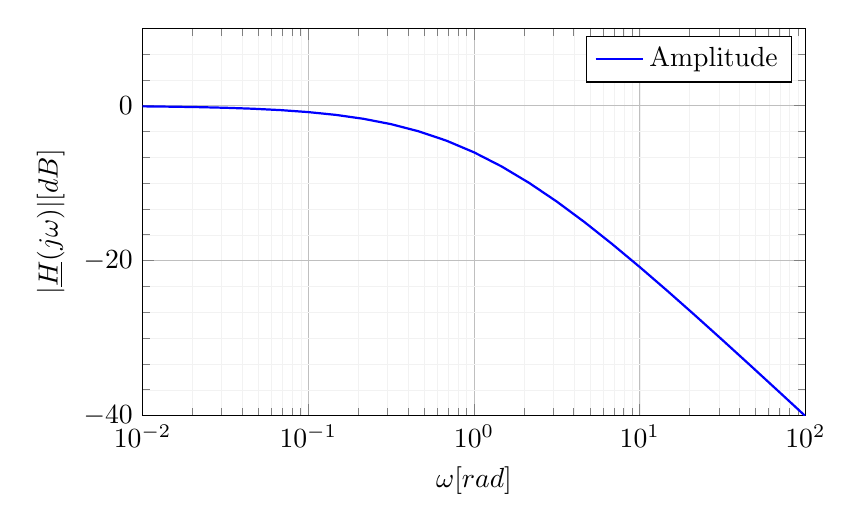
\begin{tikzpicture}
        \begin{semilogxaxis}[
            xlabel={$\omega [rad]$},
            ylabel={$|\underline{H}(j\omega)|[dB]$},
            xmin=0.01, xmax=100,
            ymin=-40, ymax=10,
            xmode=log,
            grid=both,
            grid style={line width=.1pt, draw=gray!10},
            major grid style={line width=.2pt,draw=gray!50},
            minor tick num=5,
            width=10cm,
            height=6.5cm,
            ]

            \addplot[domain=0.01:100, blue, thick] {
                20 * log10(
                1/(x+1)
                )
            };
            \addlegendentry{Amplitude};
        \end{semilogxaxis}
    \end{tikzpicture}
\end{center}
\textbf{Phasengang:}
\begin{center}
    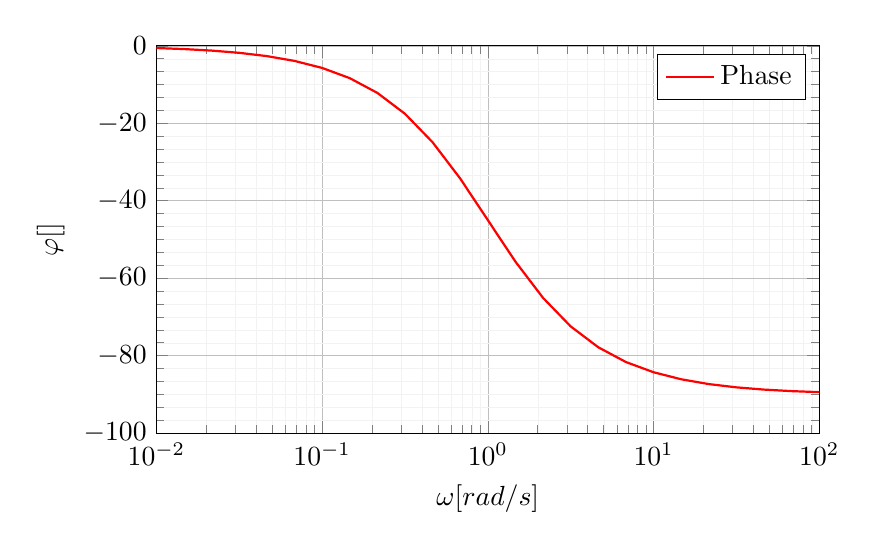
\begin{tikzpicture}
        \begin{semilogxaxis}[
                xlabel={$\omega [rad/s]$},
                ylabel={$\varphi [\degree]$},
                xmin=0.01, xmax=100,
                ymin=-100, ymax=0,
                xmode=log,
                grid=both,
                grid style={line width=.1pt, draw=gray!10},
                major grid style={line width=.2pt,draw=gray!50},
                minor tick num=5,
                width=10cm,
                height=6.5cm,
            ]

            \addplot[domain=0.01:100, red, thick] {-atan(x/1)};
            \addlegendentry{Phase};

        \end{semilogxaxis}
    \end{tikzpicture}
\end{center}

\section{Filter}
\subsection{Tiefpass}
Ein Tiefpassfilter lässt Signale mit niedrigen Frequenzen passieren, während es
Signale mit hohen Frequenzen blockiert oder abschwächt. Solche Filter können
durch LR- oder RC-Glieder aufgebaut werden.

\textbf{RC-Glied}
\begin{figure}
    \centering
    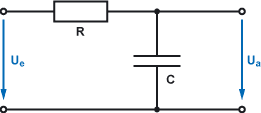
\includegraphics[width=0.5\textwidth]{LineareBauteile/RC-Glied.png}
    \caption{RC Tiefpass}
\end{figure}

\subsection{Hochpass}
\subsection{Allpass}
